\documentclass{../../../oss-ap12ibhl}

\begin{document}
%\genheader

\gentitle{9}{FLUID MECHANICS}

\begin{questions}

  \question Two blocks of different sizes and masses float in a tray of water.
  Each block is half submerged, as shown in the figure. Water has a density of
  \SI{1000}{\kilo\gram\per\metre\cubed}. What can be concluded about the
  densities of the two blocks?

  \begin{minipage}{.4\linewidth}
    \pic{1}{mc-q1}
  \end{minipage}
  \begin{minipage}{.59\linewidth}
    \begin{choices}
      \choice The two blocks have different densities, both of which are less
      than \SI{1000}{\kilo\gram\per\metre\cubed}.
      \choice The two blocks have the same density of
      \SI{500}{\kilo\gram\per\metre\cubed}.
      \choice The two blocks have the same density, but the density cannot be
      determined with the information given.
      \choice The larger block has a greater density than the smaller block, but
      the densities of the blocks cannot be determined with the information
      given.
    \end{choices}
  \end{minipage}
  \vspace{.65in}
    
  \question The figure shows four cylinders of various diameters filled to
  different heights with water. A hole in the side of each cylinder is plugged
  by a cork. All cylinders are open at the top. The corks are removed. Which of
  the following is the correct ranking of the velocity of the water ($v$) as it
  exits each cylinder?

  \begin{minipage}{.42\linewidth}
    \pic{.95}{mc-q2}
  \end{minipage}
  \begin{minipage}{.3\linewidth}
    \begin{choices}
      \choice $v_A > v_D > v_C > v_B$
      \choice $v_A = v_D > v_C > v_B$
      \choice $v_B > v_C > v_A = v_D$
      \choice $v_C > v_A = v_B = v_D$
    \end{choices}
  \end{minipage}

  \question A \SI1{\centi\metre} diameter pipe leads to a showerhead with twenty
  \SI{1}{\milli\metre} diameter exit holes. The velocity of the water in the
  pipe is $v$. What is the velocity of the water exiting the holes?
  \begin{choices}
    \choice $0.05v$
    \choice $0.5v$
    \choice $5v$
    \choice $100v$
  \end{choices}

  \uplevel{  
    \textbf{Questions \ref{cyl1} and \ref{cyl2}}

    Four differently shaped sealed containers are completely filled with
    alcohol, as shown below. Containers $A$ and $B$ are cylindrical. Containers
    $C$ and $D$ are truncated conical shapes. The top and bottom diameters of
    the containers are shown.
    \cpic{.45}{mc-q3-4}
  }
    
  \question Which of the following is the correct ranking of the pressure ($P$)
  at the bottom of the containers?
  \label{cyl1}
  \begin{choices}
    \choice $P_A = P_B = P_C = P_D$
    \choice $P_A = P_D > P_C = P_B$
    \choice $P_A > P_D > P_C > P_B$
    \choice $P_D > P_A > P_C > P_B$
  \end{choices}
    
  \question The force on the bottom of container $A$ due to the fluid inside the
  container is $F$. What is the force on the bottom of container $B$ due to
  the fluid inside?
  \label{cyl2}
  \begin{choices}
    \choice $F$
    \choice $F/4$
    \choice $F/8$
    \choice $F/16$
  \end{choices}

  \question Two cylinders filled with a fluid are connected by a pipe so that
  fluid can pass between the cylinders, as shown in the figure. The cylinder on
  the right has 4 times the diameter of the cylinder on the left. Both cylinders
  are fitted with a movable piston and a platform on top. A person stands on
  the left platform. Which of the following lists the correct number of people
  that need to stand on the right platform so neither platform moves. Assume
  that the platform and piston have negligible mass and that all the people
  have the same mass.

  \begin{minipage}{.4\textwidth}
    \pic{.95}{mc-q5}
  \end{minipage}
  \begin{minipage}{.58\textwidth}
    \begin{choices}
      \choice \num{16} people
      \choice \num{4} people
      \choice \num{1} person
      \choice It is impossible to balance the system because you need $1/16$ of
      a person on the right side.
    \end{choices}
  \end{minipage}
  \newpage
    
  \question A mass $m$ is suspended in a fluid of density $\rho$ by a string, as
  shown in the figure below. The tension in the string is $T$. Which of the
  following is an appropriate equation for the buoyancy force? Select two
  answers.
  
  \begin{minipage}{.3\textwidth}
    \pic{.95}{mc-q6}
  \end{minipage}
  \begin{minipage}{.4\textwidth}
    \begin{choices}
      \choice $F_b=mg$
      \choice $F_b=mg-T$
      \choice $F_c=a_2 \rho gh_1$
      \choice $F_d=a\rho g(h_1-h_2)$
    \end{choices}
  \end{minipage}
  
  \question Three wooden blocks of different masses and sizes float in a
  container of water, as shown in the figure. Each of the masses has a weight
  on top. Which of the following correctly ranks the buoyancy force on the
  wooden blocks?

  \begin{minipage}{.4\linewidth}
    \pic{.95}{mc-q7}
  \end{minipage}
  \begin{minipage}{.4\linewidth}
    \begin{choices}
      \choice $A > B = C$
      \choice $A = B > C$
      \choice $B > A = C$
      \choice $B > A > C$
    \end{choices}
  \end{minipage}
    
  \question Two blocks of the same dimensions are floating in a container of
  water, as shown in the figure. Which of the following is a correct statement
  about the two blocks?

  \begin{minipage}{.4\linewidth}
    \pic{.95}{mc-q8}
  \end{minipage}
  \begin{minipage}{.58\linewidth}
    \begin{choices}
      \choice The net force on both blocks is the same.
      \choice The buoyancy force exerted on both blocks is the same.
      \choice The density of both blocks is the same.
      \choice The pressure exerted on the bottom of each block is the same.
    \end{choices}
  \end{minipage}
  \vspace{.3in}
    
  \question The figure shows four cubes of the same volume at rest in a
  container of water. Cube $C$ is partially submerged. Cubes $A$, $B$, and $D$
  are fully submerged, with $B$ resting on the bottom of the container. Which
  of the following correctly ranks the densities ($\rho$) of the cubes? Assume
  the water to be incompressible.

  \begin{minipage}{.4\linewidth}
    \pic{.95}{mc-q9}
  \end{minipage}
  \begin{minipage}{.4\linewidth}
    \begin{choices}
      \choice $\rho_C >\rho_D >\rho_A >\rho_B$
      \choice $\rho_B >\rho_A >\rho_D >\rho_C$
      \choice $\rho_B >\rho_A =\rho_D >\rho_C$
      \choice $\rho_B >\rho_A =\rho_D =\rho_C$
    \end{choices}
  \end{minipage}
    
  \question A beaker of water sits on a balance. A metal block with a mass of
  \SI{70}{\gram} is held suspended in the water by a spring scale in position
  1, as shown. In this position, the reading on the balance is
  \SI{1260}{\gram}, and the spring scale reads \SI{120}{\gram}. When the block
  is lifted from the water to position 2, what are the readings on the balance
  and spring scale?

  \begin{minipage}{.28\linewidth}
    \pic{.7}{mc-q10}
  \end{minipage}
  \begin{minipage}{.4\linewidth}
    \begin{tabular}{c c c}
      & \underline{\textbf{Balance reading}} &
      \underline{\textbf{Spring scale reading}}\\
      (A) & \SI{1190}{\gram} & \SI{120}{\gram}\\
      (B) & \SI{1190}{\gram} & \SI{190}{\gram}\\
      (C) & \SI{1260}{\gram} & \SI{120}{\gram}\\
      (D) & \SI{1330}{\gram} & \SI{120}{\gram}
    \end{tabular}
  \end{minipage}
    
  \question Blood cells pass through an artery that has a buildup of plaque
  alon both walls, as shown in the figure. Which of the following correctly
  describes the behavior of the blood cells as they move from the right side of
  the figure through the area of plaque? Assume the blood cells can change
  volume.
  
  \begin{minipage}{.4\linewidth}
    \pic{.9}{mc-q11}
  \end{minipage}
  \begin{minipage}{.57\linewidth}
    \begin{choices}
      \choice The blood cells increase in speed and expand in volume.
      \choice The blood cells increase in speed and decrease in volume.
      \choice The blood cells decrease in speed and expand in volume.
      \choice The blood cells decrease in speed and decrease in volume.
    \end{choices}
  \end{minipage}
  \newpage
  
  \question Firefighters use a hose with a 2 cm exit nozzle connected to a
  hydran with an 8 cm diameter opening to attack a fire on the second floor of a
  building 6 m above the hydrant, as shown in the figure. What pressure must
  be supplied at the hydrant to produce an exit velocity of
  \SI{15}{\metre\per\second}? (The density of water is
  \SI{1000}{\kilo\gram\per\metre\cubed}, and the exit pressure is
  \SI{1e5}{\pascal}.)
  
  \begin{minipage}{.4\linewidth}
    \pic{.95}{mc-q12}
  \end{minipage}
  \begin{minipage}{.4\linewidth}
    \begin{choices}
    \choice\SI{1.7e5}\pascal
    \choice\SI{2.0e5}\pascal
    \choice\SI{2.6e5}\pascal
    \choice\SI{3.2e5}\pascal
    \end{choices}
  \end{minipage}

  % THIS TAKEN FROM THE 2001 AP PHYSICS B EXAM FREE-RESPPONSE QUESTION #5
  \uplevel{
    \centering
    \pic{.5}{submerged-block}
    
    \underline{Note:} Figure not drawn to scale.
  }

  \question A large rectangular raft (density
  \SI{650}{\kilo\gram\per\metre\cubed}) is floating on a lake. The surface area
  of the top of the raft is \SI{8.2}{\metre\squared} and its volume is
  \SI{1.80}{\metre\cubed}. The density of the lake water is
  \SI{1000}{\kilo\gram\per\metre\cubed}.
  \begin{parts}
    \part Calculate the height $h$ of the portion of the raft that is above the
    surrounding water.
    
    \part Calculate the magnitude of the buoyant force on the raft and state its
    direction.
    
    \part If the average mass of a person is \SI{75}{\kilo\gram}, calculate the
    maximum number of people that can be on the raft without the top of the
    raft sinking below the surface of the water. (Assume that the people are
    evenly distributed on the raft.)
  \end{parts}
  \newpage
  
  % THIS IS TAKEN FROM THE 2012 AP PHYSICS B EXAM FREE-RESPPONSE QUESTION #3
  \uplevel{
    \cpic{.35}{oils}
  }
  \question A glass U-tube with a uniform diameter of 0.850 cm is used to
  determine the density of an oil. As shown in the figure above, a 24.5 cm
  column of water balances a 27.2 cm column of the oil so that interfaces $A$
  and $B$ of the mercury with the other liquids are at the same height. The
  density of water is \SI{1.00e3}{\kilo\gram\per\metre\cubed}.
  \begin{parts}
    \part Calculate the density of the oil.

    \part Calculate the absolute pressure at $B$, the interface between the
    water and the mercury.
    
    \uplevel{  
      \cpic{.3}{u-tube}
      A new tube, identical to the U-tube except for a cone shape on the left,
      as shown above, is filled with the same volume of mercury that was in the
      U-tube. The mercury is at the same height on both sides of the new tube
      as it was in the U-tube, as shown by the dashed line. The same volumes of
      oil and water that were in the U-tube are now poured into the new tube,
      on the left and right respectively.
    }

    \part Indicate the new position of $B$ relative to $A$. Justify your answer.
    
    \vspace{.1in}
    \underline{\hspace{.3in}} Above $A$\hspace{.2in}
    \underline{\hspace{.3in}} Below $A$\hspace{.2in}
    \underline{\hspace{.3in}} At the same height as $A$
    \vspace{.1in}
      
    \part A small piece of wood with density less than that of the oil is placed
    so that it floats in the left side of the tube. Indicate whether the
    pressure at the bottom of the tube increases, decreases, or remains the
    same.

    \vspace{.1in}
    \underline{\hspace{.3in}} Increases\hspace{.2in}
    \underline{\hspace{.3in}} Decreases\hspace{.2in}
    \underline{\hspace{.3in}} Remains the same
  \end{parts}
  \newpage
  
  % THIS IS TAKEN FROM THE 2014 AP PHYSICS B EXAM FREE-RESPONSE QUESTION #2
  \uplevel{
    \centering
    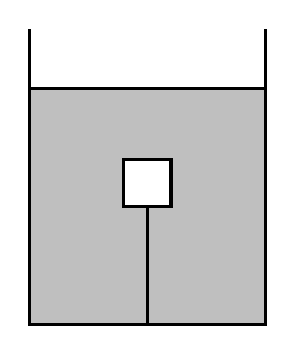
\begin{tikzpicture}[scale=1.5]
      \fill[gray!50](0,0) rectangle(2,2);
      \draw[very thick](0,2.5)--(0,0)--(2,0)--(2,2.5);
      \draw[very thick](0,2)--(2,2);
      \draw[very thick](1,0)--(1,1);
      \draw[very thick,fill=white](.8,1) rectangle(1.2,1.4);
    \end{tikzpicture}
  }
  
  \question A cube of mass $m$ and side length $L$ is completely submerged in a
  tank of water and is attached to the bottom of the tank by a string, as shown
  above. The tension in the string is 0.25 times the weight of the cube. The
  density of water is \SI{1000}{\kilo\gram\per\metre\cubed}.
  \begin{parts}
    \part On the dot below that represents the cube, draw and label the forces
    (not components) that act on the cube while it is attached to the string.
    Each force must be represented by a distinct arrow starting on, and pointing
    away from, the dot.
    \begin{center}
      \vspace{.5in}
      \tikz{\fill(0,0) circle(.25);}
      \vspace{.5in}
    \end{center}
    
    \part Calculate the density of the cube.

    \part The string is now cut. Calculate the magnitude of the acceleration of
    the cube immediately after the string is cut. If you need to draw anything
    other than what you have shown in part (a) to assist in your solution, use
    the space below. Do NOT add anything to the figure in part (a).
    
    \part Indicate whether the magnitude of the buoyant force on the cube
    increases, decreases, or remains the same while the cube is rising, but
    before it reaches the surface. Justify your answer.

    \vspace{.1in}
    \underline{\hspace{.3in}} Increases\hspace{.2in}
    \underline{\hspace{.3in}} Decreases\hspace{.2in}
    \underline{\hspace{.3in}} Remains the same
  \end{parts}
  \newpage

  \uplevel{
    \cpic{.38}{fr-q2}
  }
  
  \question A \SI{1.}{\centi\metre} radius hose with a \SI{.50}{\centi\metre}
  radius exit nozzle is being used to fill a \SI{1000}{\milli\litre} beaker
  with oil (\SI{1000}{\milli\litre}=\SI{.0010}{\metre\cubed}). The velocity of
  the oil in the hose is $\varv=\SI{0.40}{\metre\per\second}$ as shown in the
  figure. The density of the oil is \SI{960}{\kilo\gram\per\metre\cubed}, and
  the atmospheric pressure is \SI{1.01e5}\pascal.
  
  \begin{parts}
    \part The nozzle attached to the end of the hose has a smaller radius than
    the hose. If the nozzle is removed from the hose, will the beaker be filled
    faster? Justify your answer with conservation laws.
    
    \part Calculate the exit velocity of the oil from the nozzle.
    
    \part How long will it take to fill the beaker?
    
    \part Point A is shown in the figure. How does the pressure in the fluid at
    point A compare to the pressure in the fluid at the exit nozzle? Justify
    your claim.
    
    \part The hose is now used to fill a \SI{200}{\milli\litre} graduated
    cylinder with oil to the same height as the height of the oil in the
    \SI{1000}{\milli\litre} beaker. Compare the net force from the oil on the
    bottom of the \SI{200}{\milli\litre} cylinder and the
    \SI{1000}{\milli\litre}. Explain your answer.
  \end{parts}
  \newpage

  \uplevel{
    \cpic{.27}{fr-2a}
  }
  
  \question A cube of lead with a side dimension of \SI{5.}{\centi\metre} is
  slowly lowered into the beaker of oil by a thin string attached to a spring
  scale at a constant rate, as shown above. The density of lead is
  \SI{11300}{\kilo\gram\per\metre\cubed}.
  
  \begin{parts}
    \part What will be the spring scale reading in newtons when the lead has
    been submerged to location 2?
    
    \part Does the spring scale reading increase, decrease, or stay the same
    when the cube is lowered from location 2 to location 3? Justify your
    answer by referencing the pressure of the fluid on the lead cube.
    
    \part The lead cube is lowered from above the oil's surface (location 1) to
    a spot just below the surface (location 2) until the cube is just above
    the bottom of the beaker (location 3). Describe any changes in pressure
    on the bottom of the beaker during this process. Explain your answer.
  \end{parts}
\end{questions}
\end{document}
